% !TeX root = Bericht.tex
% !TeX spellcheck = de_DE
\section{Results}
We start by filtering out emission lines with an effective width of $EW_\lambda > 0.12 \unit{\angstrom}$ and where the fitted peak was shifted more than $\delta\lambda = 0.15 \unit{\angstrom}$ from the theoretical value, since this is the detectors resolution limit. We are left with 154 datapoints, which according to \autoref{eqn:line} should follow a linear behaviour. In order to determine the last unknown variables in \autoref{eqn:line} (the effective temperature $T$ and the iron-to-hydrogen ratio $N_{\text{Fe}}/N_{\text{H}}$) we fit a linear function. In \autoref{fig:plot1} both data and fitfunction can be seen. 

\begin{figure}[H]
	\centering
	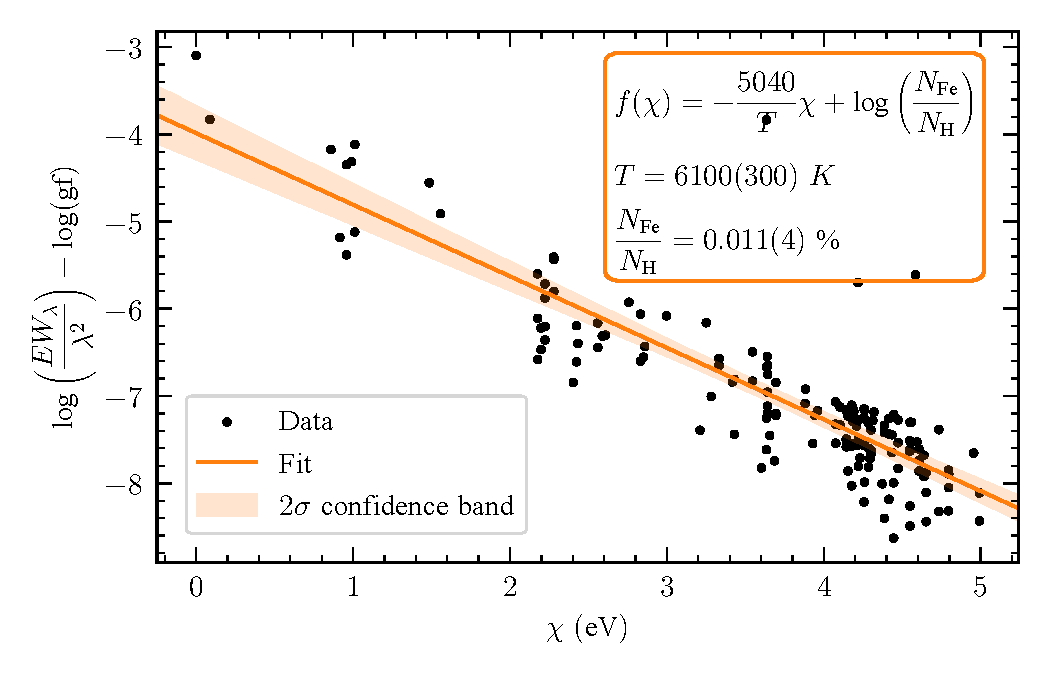
\includegraphics[width=\textwidth]{fit.pdf}
	\caption{The data is plotted against the excitation energy $\chi$ in such a way as to make extraction of the effective temperature $T$ and iron-to-hydrogen ratio $\NFe/\NH$ possible via a linear fit. This can be seen in orange, accompanied by a $2\sigma$ confidence band. The analytical function and the resulting parameters are shown on the top right corner.}
	\label{fig:plot1}
\end{figure}

As one can see in \autoref{fig:plot1}, a linear behaviour can be observed in the data, albeit with noticeable dispersion. The uncertainty of the measurements are not included since they can not be estimated in a meaningful way. Nevertheless we get a first estimate for the effective temperature of the sun and the relative iron abundance (compared to hydrogen) in the sun's atmosphere. When comparing our results
\[ T = 6100(300) \unit{K} \qquad \frac{\NFe}{\NH} = 0.011(4) \unit{\percent} \]
with literature values \autocite{NASA}
\[ T_{\text{lit}} = 5772 \unit{K} \qquad \frac{\NFe}{\NH} = 0.0043 \unit{\percent} \]
we can observe deviations of multiple sigma. One possible error source lies in the used data. The linear relation in is only valid for absorption lines, for which the effective width is proportional to the wavelength. 

To investigate this further, we proceed by plotting the curve of growth, which can be seen in \autoref{fig:plot2}. The data is plotted such that theory predicts a trend following a line with slope 1 (\ang{45}). To not distort the chosen representation the axes were set to a 1:1 aspect ratio.
\begin{figure}[H]
	\centering
	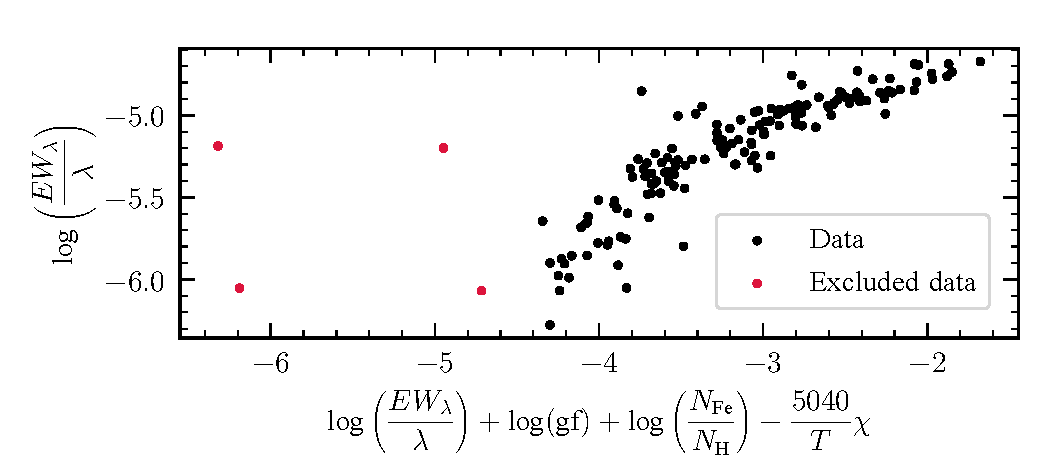
\includegraphics[width=\textwidth]{exclude.pdf}
	\caption{The curve of growth of all data points is plotted. The data was treated in such a way, as to make the expected behaviour a line with \ang{45} angle, when using an 1:1 axis aspect ratio. 3 anomalous datapoints were identified (marked red) and will be excluded from further analysis.}
	\label{fig:plot2}
\end{figure}
We identify 3 anomalous datapoints that clearly do not follow the expected trend. We therefore exclude these from further analysis and proceed by plotting the refined data (\autoref{fig:plot3}) in the same manner as in \autoref{fig:plot2}. Again, the axis aspect ratio was chosen to be equal. This allows us to plot a line with \ang{45} incline (dashed gray line in \autoref{fig:plot2}). The offset was manually chosen to take the (somewhat arbitrary) value of $-1.7$. This  is not too important since it is not used for quantitative reasons but only aids in distinguishing between different behaviour regimes. 

\begin{figure}[H]
	\centering
	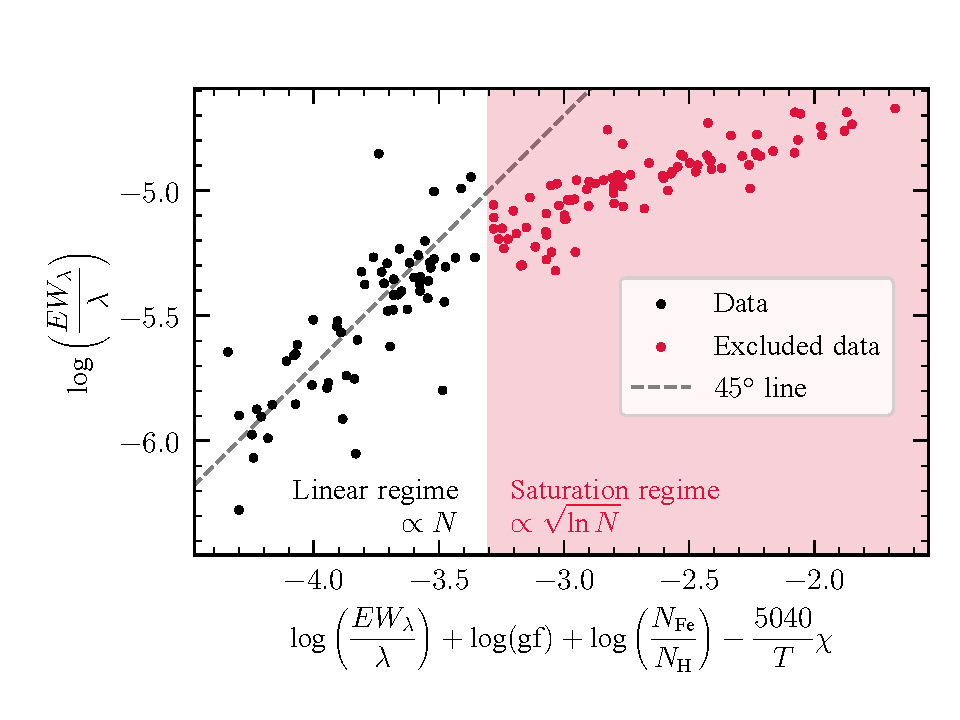
\includegraphics[width=\textwidth]{exclude2.pdf}
	\caption{The curve of growth of refined data is plotted. The data was treated in such a way, as to make the expected behaviour a line with \ang{45} angle (dashed gray), when using an 1:1 axis aspect ratio. The plot can roughly be divided into two regimes with different proportionality behaviour, marked accordingly.}
	\label{fig:plot3}
\end{figure}

As shown in \autoref{fig:plot3} we can divide the data into a region where the effective width is proportional to $N_i$ and the saturation regime, where is scales with $\sqrt{\ln N_i}$. The dividing line was chosen manually and can be somewhat motivated by the observation that left of the red line there is an equal amount of datapoints of both sides of the theoretical trend (dashed line), whilst in the saturation regime all datapoints are below the \ang{45} line.

Now we can go back to estimating $T$ and $\NFe/\NH$ with the reduced data. This is can be seen in \autoref{fig:plot4}. Additionally the linear fit to the entire data as seen in \autoref{fig:plot1}) is plotted as dashed gray line.

\begin{figure}[H]
	\centering
	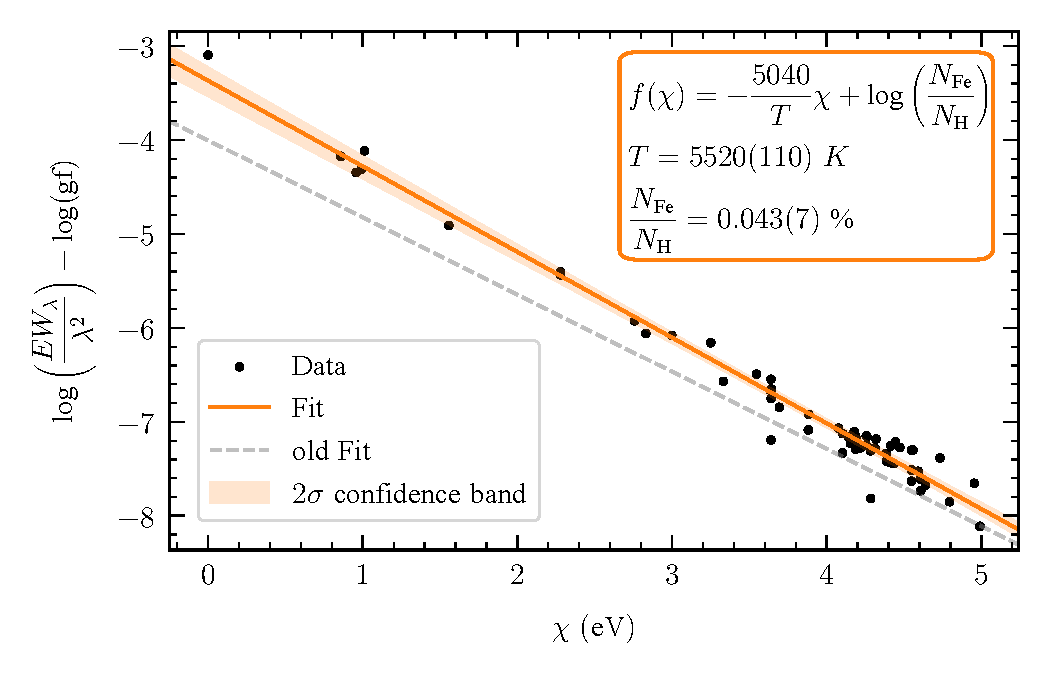
\includegraphics[width=\textwidth]{fit2}
	\caption{The data is plotted against the excitation energy $\chi$ in such a way as to make extraction of the effective temperature $T$ and iron-to-hydrogen ratio $\NFe/\NH$ possible via a linear fit. This can be seen in orange, accompanied by a $2\sigma$ confidence band. The analytical function and the resulting parameters are shown on the top right corner. Additionally the linear fit to all data (from \autoref{fig:plot1}) is plotted as dashed gray line.}
	\label{fig:plot4}
\end{figure}

One can see the effect of excluding emission lines from the saturation regime. Both, slope and y-intercept have changed compared the fit to all data. We get the following values out of the fit:
\[ T = 5520(110) \unit{K} \qquad \frac{\NFe}{\NH} = 0.043(7) \unit{\percent}. \]
When comparing to the literature values mentioned above, we can see that our temperature estimate has improved somewhat, going from $\approx 400 \unit{K}$ to $\approx 200 \unit{K}$ deviation. The iron abundance has gotten worse, with the estimate lying squarely one order of magnitude above the literature value. The data refinement hast visually improved the plots, with data showing a clearer linear behaviour with less scatter. The quantitative results however do not show a clear improvement compared to unfiltered data. This indicates that there are systematic errors that dominate over the introduced by using saturated absorption lines. The weather and more generally the earths atmosphere could have an impact on the measurements if the effective width of absorption peaks is not influenced equally for all wavelengths. 